% This template is provided for all the participants of the seminar ``Text Mining''
%%%%%%%%%%%%%%%%%%%%%
% Author information:
%%%%%%%%%%%%%%%%%%%%%
% Jannik Strötgen
% Institute of Computer Science
% Database Systems Research Group
% INF 348 
% 69120 Heidelberg
% stroetgen@uni-hd.de
%%%%%%%
% Date: April 24, 2010
%%%%%%% 

\documentclass[
     11pt,         % font size
     a4paper,      % paper format
     oneside,
     ]{article}

%%%%%%%%%%%%%%%%%%%%%%%%%%%%%%%%%%%%%%%%%%%%%%%%%%%%%%%%%%%%

% PACKAGES:

% Use German :
\usepackage[USenglish, ngerman]{babel}
% Input encoding
\usepackage[utf8]{inputenc}
% Font encoding
\usepackage[T1]{fontenc}
% Einbinden von URLs:
\usepackage{url}
% Include Graphic-files:
\usepackage{graphicx}
% Include PDF links
%\usepackage[pdftex, bookmarks=true]{hyperref}
% Fuer Textsatz
\usepackage{setspace}
% For bibliography style
\usepackage[numbers]{natbib}
% for Latex symbols
\usepackage{doc}
%amsmath
\usepackage{amsmath}
\usepackage{amsthm}
%booktabs
\usepackage{booktabs}
%SI-Einheiten
\usepackage{siunitx}

%%%%%%%%%%%%%%%%%%%%%%%%%%%%%%%%%%%%%%%%%%%
% Titel, Autor, Seminar, Semester, Dozent %
%%%%%%%%%%%%%%%%%%%%%%%%%%%%%%%%%%%%%%%%%%%
\newcommand{\mytitle}{Coreference of Named Entities}
\newcommand{\myauthor}{Philipp Schäfer, Daniel Kruck}
\newcommand{\myseminar}{Text Mining}
\newcommand{\mysemester}{Sommersemester 2010}
\newcommand{\mydozent}{Jannik Strötgen}
\newcommand{\mydozentTwo}{Prof. Dr. Michael Gertz}



\newtheoremstyle{custm}% name of the style to be used
  {}% measure of space to leave above the theorem. E.g.: 3pt
  {}% measure of space to leave below the theorem. E.g.: 3pt
  {}% name of font to use in the body of the theorem
  {0em}% measure of space to indent
  {\bf }% name of head font
  {}% punctuation between head and body
  {0.5cm}% space after theorem head; " " = normal interword space
  {}% Manually specify head

\theoremstyle{custm}

\newtheorem*{thm_defi}{Definition:}
\newenvironment{defi} [1][]{\begin{thm_defi} {\underline{\textbf{#1}}\ \\}}{\end{thm_defi} }


% OTHER SETTINGS:
\setlength{\parindent}{0in}

% Pagestyle:
\pagestyle{myheadings}
\markright{\myauthor: \mytitle}

\begin{document}

%%%%%%%%%%%%%%%%%%%%%%%%%%%%%%%%%%%%% <TITLE> %%%%%%%%%%%%%%%%%%%%%%%%%%%%%%%%%%%%%
\pagenumbering{roman}
\begin{titlepage}
\begin{tabular}[l]{l}
% Angaben zum Seminar
Ruprecht-Karls-Universität Heidelberg\\
Institut für Informatik\\
\mysemester\\
Seminar: \myseminar\\
Dozenten: \mydozent\\
\phantom{Dozenten: }\mydozentTwo\\
\end{tabular}

\vspace{4cm}
\begin{center}
\textbf{\large Seminararbeit} % Proseminararbeit,Studienarbeit, Interdisziplinaeres Projekt
\vspace{0.5\baselineskip}

% Titel wird ausgegeben (siehe oben)
{\huge
\mytitle
}
\end{center}

\vfill 
% Persönliche Angaben
\begin{tabular}[l]{ll}
Name:           & \myauthor\\
Matrikelnummer: & 2612579 (Philipp), 2440234 (Daniel)\\
Studiengang:    & Angewandte Informatik (6. Semester)\\
Email: & trashzopf@googlemail.com (Philipp), daniel.kruck@gmx.net (Daniel)\\
Datum der Abgabe: & \today \\
\end{tabular}

\end{titlepage}
%%%%%%%%%%%%%%%%%%%%%%%%%%%%%%%%%%%%% </TITLE> %%%%%%%%%%%%%%%%%%%%%%%%%%%%%%%%%%%%

% Zeilenabstand
\onehalfspacing

\newcommand{\NaNg}{``A 2-Poisson Model for Probabilistic Coreference of Named Entities for Improved Text Retrieval''}


%%%%%%%%%%%%%%%%%%%%%%%%%%%%% <Antiplagiatserklärung> %%%%%%%%%%%%%%%%%%%%%%%%%%%%%
\thispagestyle{empty}
\vspace*{100pt}
Hiermit versichere ich \textbf{\myauthor}, dass ich die Hausarbeit mit dem Titel \textbf{\mytitle}
im Seminar \textbf{\myseminar}
im \textbf{\mysemester}
bei \textbf{\mydozent} und \textbf{\mydozentTwo}
selbstständig und nur mit den in der Arbeit angegebenen Hilfsmitteln verfasst habe.
Zitate sowie der Gebrauch fremder Quellen, Texte und Hilfsmittel habe ich nach den
Regeln wissenschaftlicher Praxis eindeutig gekennzeichnet. 
Mir ist bewusst, dass ich
fremde Texte und Textpassagen nicht als meine eigenen ausgeben darf und dass ein
Verstoß gegen diese Grundregel des wissenschaftlichen Arbeitens als Täuschungs- und
Betrugsversuch gilt, der entsprechende Konsequenzen nach sich zieht. Diese bestehen
in der Bewertung der Prüfungsleistung mit "nicht ausreichend" (5,0) sowie ggf. weiteren
Maßnahmen.

Außerdem bestätige ich, dass diese Arbeit in gleicher oder ähnlicher Form noch in keinem anderen Seminar vorgelegt wurde.
\vspace*{50pt}

Heidelberg, den \today \hspace{2cm} \underline{\phantom{Platz für die Unterschrift}}
\newpage
%%%%%%%%%%%%%%%%%%%%%%%%%%%%% </Antiplagiatserklärung> %%%%%%%%%%%%%%%%%%%%%%%%%%%%



%%%%%%%%%%%%%%%%%%%%%%%%%%%%%% <Inhaltsverzeichnis> %%%%%%%%%%%%%%%%%%%%%%%%%%%%%%%
% Table of contents
\tableofcontents
\newpage
%%%%%%%%%%%%%%%%%%%%%%%%%%%%%% </Inhaltsverzeichnis> %%%%%%%%%%%%%%%%%%%%%%%%%%%%%%





%%%%%%%%%%%%%%%%%%%%%%%%%%%%% <Hauptteil der Arbeit> %%%%%%%%%%%%%%%%%%%%%%%%%%%%%%
\pagenumbering{arabic}

%%%%%%%%%%%%%%%%%%%%%%%%%%%%% <Einleitung> %%%%%%%%%%%%%%%%%%%%%%%%%%%%%%%%%%%%%%%%
\section{Einleitung}
In letzter Zeit hat sich das Sortier- und Suchverhalten der Menschheit geändert. Sortierte man früher noch seine Dokumente in Ordner, ist man heute glücklich, wenn man mit leistungsstarken Suchalgorithmen schnell und präzise das gewünschte Dokument findet.\\
Dabei beschränken sich Suchanfragen nicht nur auf lokale Daten, sondern werden sogar großteils ans Web gestellt. Eine häufige Anfrageform an Suchmaschinen sind hierbei die \textit{named entity queries}\cite{paper:Guha}.\\
\begin{table}[h]
	\centering
	\begin{tabular}{c}
		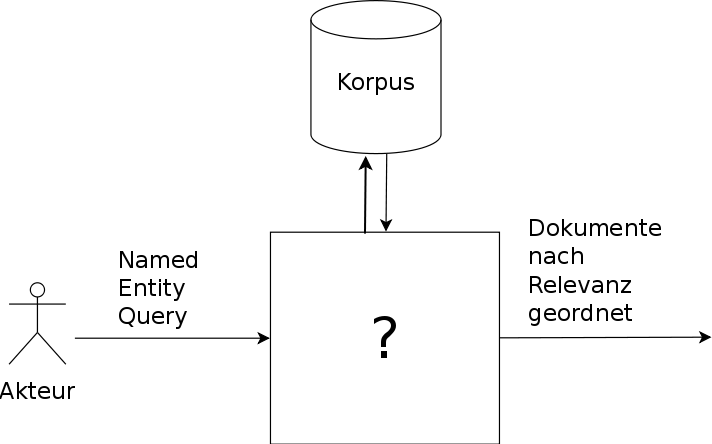
\includegraphics[scale=.2]{pics/overview}
	\end{tabular}
	\caption{Häufige Suchanfrage an Suchmaschinen}
	\label{tab:freq_query}
\end{table}\\
Ein Problem bei solchen Suchanfragen ist es, die Häufigkeit der \textbf{named entity} in Dokumenten richtig zu erfassen\cite{paper:Na}.
Denn die Referenzierung des Objektes, das sich hinter einem Eigennamen verbirgt, wird sowohl mit dem Eigennamen selbst, als auch mit kompakteren Ausdrücken vorgenommen.\\
So wird beispielsweise in einem Text, der von Peter Chen handelt, die Person \textit{Peter Chen} auch mit \textit{"`er"'} referenziert.\\
\\
\fbox{ 
\begin{minipage}{12cm}
	"`\textbf{Chen} has recieved serveral awards in the fields of Information Technology. \textbf{He} received the Data Resource Management Technology Award [\ldots]"' \cite{wiki:peter_chen}
\end{minipage}
}\\
\\
In der folgenden Hausarbeit wird ein statistisches Verfahren erklärt, welches die Häufigkeit von Eigennamen in Dokumenten schätzen soll. Grundlage für diese Ausarbeitung ist ein Paper der Herren Na und Ng über "`A 2-Poisson Model for Probabilistic Coreference of Named Entities for Improved Text Retrieval"'\cite{paper:Na}.



%%%%%%%%%%%%%%%%%%%%%%%%%%%%% <Coreferentially Enhanced Entity Frequency (CEEF)> %%
\section{Co-referentially Enhanced Entity Frequency (CEEF)}
%%%%%%%%%%%%%%%%%%%%%%%%%%%%% <CEEF - Basic> %%%%%%%%%%%%%%%%%%%%%%%%%%%%%%%%%%%%%%
\subsection{Plausible Annahme über die Verteilung von Koreferenzen}
%PDF-Features von latex nachlesen; wir bräuchten einen link auf die Einleitung - und zwar auf die fbox
Die Häufigkeit von Eigennamen in Dokumenten ist schwer zu erfassen. Zählt man nur die \textit{named entites} selbst, erhält man die raw entity frequency:
\[tf\left( e;d \right)=\sharp \text{(named entity)}\]
Die raw entity frequency beachtet  noch keine zusätzlichen Koreferenzen auf das Objekt hinter dem gesuchten Eigennamen. Um später ein besseres Ranking ausführen zu können, möchten wir möglichst alle Referenzen erfassen. Also addieren wir die Häufigkeit der Koreferenzen zu unserer raw entity frequency:
\[tf\left( e;d \right)\leq tf_{true}\left( e;d \right)=tf\left( e;d \right)+\underbrace{atf(e_Q;A,d)}_{Korefernzen}\]
Theoretisch sind wir nun am Ziel. Praktisch ist es aber nicht so einfach, die Häufigkeit der Koreferenzen zu bestimmen. Mit Programmen, die Koreferenzen vollständig auflösen, geht ein überdimensionaler Berechnungsaufwand einher. Zudem sind diese Programme noch nicht besonders Präzise und ordnen weniger als 70\% der Koreferenzen richtig zu.\cite{paper:Na}
\\
Seung-Hoon Na und Hwee Tou Ng untersuchteni deswegen einen statistischen Ansatz zur Schätzung der Koreferenzen. Dafür nehmen sie folgendes an:
\fbox{ 
\begin{minipage}{12cm}
	``Our key assumption is that the frequency of anaphoric expressions is distributed over named entities in a document according to the probabilities of whether the document is elite for the named entities.''\cite{paper:Na}
\end{minipage}
}\\


%%%%%%%%%%%%%%%%%%%%%%%%%%%%% <CEEF - Formalisierung> %%%%%%%%%%%%%%%%%%%%%%%%%%%%%
\subsection{Formalisierung}
Bevor wir zur eigentlichen Statistik kommen, legen wir noch die mathematische Schreibweise für diese Aufgabe fest.
Zunächst sei Q unsere query. 

 \begin{itemize}
	\item $Q$ = query (Suche)
	\item $e_Q$ = query entity (gesuchte Entität)
	\item $e_N$ = non-query entity
	\item $A$ = Menge plausibler anaphorischer Ausdrücke
	\item $tf(A;d)$ = Anzahl von $A$ in Dokument $d$
	\item $\varepsilon (A;d)$ = Menge plausibler Entitäten in Dokument $d$
	\item $tf(e;d)$ = raw entity frequency
	\item $atf(e;A,d)$ = anaphoric entity frequency
  \end{itemize}



%%%%%%%%%%%%%%%%%%%%%%%%%%%%% <CEEF - Eliteness> %%%%%%%%%%%%%%%%%%%%%%%%%%%%%%%%%%%
\subsection{Eliteness}

\begin{defi}
	A document is \underline{elite} for a term if the document is ``about'' the concept represented by the term \cite{paper:Robertson}.
\end{defi}


Bei genauerer Begutachtung der Definition liegt die grundlegende Annahme von Seung-Hoon Na und Hwee Tou Ng, dass die Bezüge der anaphorischen Ausdrücke auf die Entitäten im Zusammenhang stehen, ob ein Dokument bezüglich dieser Entität „elite“ ist, oder nicht, nahe. Wir definieren uns also einen weiteren Faktor:

\begin{defi}
$P(\textbf{E}(e) = 1 | d)$ ist die Wahrscheinlichkeit, dass ein Dokument für eine Entität $e$ „elite“ ist.
\end{defi}

Jetzt können wir folgendes setzen:

\begin{equation}
P(e_Q | A,d) = \frac{P(\textbf{E}(e) = 1 | d)}{\sum_{e \in \varepsilon (A;d)} P(\textbf{E}(e) = 1 | d)}
\end{equation}
Wir machen also nichts anderes, als die Wahrscheinlichkeit der Eliteness des Dokumentes bezogen auf unsere gesuchte Entität in Relation mit den Wahrscheinlichkeiten der anderen Named Entities zu stellen.\\
Jetzt vereinfachen wir die Formel noch ein wenig, indem wir zuerst alle non-query Entitäten nach der Wahrscheinlichkeit der Eliteness sortieren. Danach werden die $K$ non-query Entitäten mit der höchsten Wahrscheinlichkeit selektiert, sodass sich unsere Formel auf Folgendes beschränkt:

\[ P(e_Q | A,d) \approx \frac{P(\textbf{E}(e) = 1 | d)}{P(\textbf{E}(e) = 1 | d) + \sum_{i=1}^{K} P(\textbf{E}(e_{n}^{(i)}) = 1 | d)} \]

$K$ ist in dem Fall frei gewählt und kann entsprechend angepasst werden. So dass tatsächlich nur Wahrscheinlichkeiten vernachlässigt werden, die nicht ins Gewicht fallen.\\
Nun suchen wir uns eine repräsentative non-query Entität heraus und setzen die Wahrscheinlichkeit der Eliteness aller anderen der Top-$K$ Entitäten mit der Wahrscheinlichkeit der Herausgesuchten gleich. Somit erhalten wir eine stark vereinfachte, aber trotzdem recht genaue Alternative von $(1)$.

\[ P(e_Q | A,d) \approx \frac{P(\textbf{E}(e) = 1 | d)}{P(\textbf{E}(e) = 1 | d) + K \cdot P(\textbf{E}(e_N) = 1 | d)} \]


Im Folgenden gilt es also, den Faktor $P(\textbf{E}(e) = 1 | d)$ zu berechnen.




%%%%%%%%%%%%%%%%%%%%%%%%%%%%% <CEEF - Poisson> %%%%%%%%%%%%%%%%%%%%%%%%%%%%%%%%%%%%
\subsection{Poisson}


%%%%%%%%%%%%%%%%%%%%%%%%%%%%% <Zusätzliche Schritte> %%%%%%%%%%%%%%%%%%%%%%%%%%%%%%
\section{Zusätzliche Bearbeitungsschritte}

%%%%%%%%%%%%%%%%%%%%%%%%%%%%% <Automatische Klassifizierung der NE> %%%%%%%%%%%%%%%
\subsection{Automatische Klassifizierung der named entities}
Nachdem man nun die Wahrscheinlichkeit schätzen kann, mit der ein Dokument ``elite'' ist, benötigt man nun noch die Häufigkeit der möglichen Koreferenzen.\\
Dafür müssen wir zunächst herausbekommen, von welchem Typ die Entity Query ist. Für Personen wird
\[A_P=\left\{ \text{'he', 'she', 'his', 'her', 'himself', 'herself'} \right\}\]
als sinnvolle Menge von Koreferenzen angesehen. Für Objekte wird eine erweiterbare Menge an Koreferenzen um
\[A_0=\left\{ \text{'it', 'its', \dots} \right\}\]
bei Bedarf verwendet. Das hat den Grund, dass Objekte oft mit Nomen referenziert werden. So wird beispielsweise ``Google'' eventuell mit ``Suchmaschine'', ``Internetriese'' oder ähnlichem bezeichnet.\\
\\
Für die Unterscheidung zwischen Person und Objekt wird ein Support Vector Machine Klassifikator eingesetzt.\\
Dafür werden zunächst Entitäten aus einer Trainingsmenge betrachtet. Bei diesen Eigennamen wird dem Computer als zusätzliche Information mitgeteilt, ob es sich um eine Person oder um ein Objekt handelt. Der Computer sucht dann die besten M Treffer zu den jeweiligen Eigennamen heraus und errechnet charakteristische Werte für diesen Eigennamen. Da wir hier herausbekommen wollen, ob es sich um ein Objekt oder um eine Person handelt, werden bei den Top M Einträgen die Koreferenzen betrachtet. Kommt häufig $A_P=\left\{ \text{'he', 'she', 'his', 'her', 'himself', 'herself'} \right\}$ vor, so wird es wahrscheinlicher, dass es sich die betrachtete Entität eine Person ist. Kommt $A_0=\left\{ \text{'it', 'its'} \right\}$ häufig vor, so handelt es sich wahrscheinlich um ein Objekt. Die Quantifizierung erfolgt normiert nach:
\[f_P\left( Q \right)=\frac{1}{|F\left( Q \right)|}\sum_{d\in F\left( Q \right)} \frac{tf\left( A_P;d \right)}{len \left( d \right)}\]
\[f_O\left( Q \right)=\frac{1}{|F\left( Q \right)|}\sum_{d\in F\left( Q \right)} \frac{tf\left( A_O;d \right)}{len \left( d \right)}\]
Dabei stellt $F\left( Q \right)$ die Menge der besten M Treffer dar, $|F\left( Q \right)|$ die Kardinalität dieser Menge, $tf\left( A_P;d \right)$ die Häufigkeit der Koreferenzen auf Personen in dem jeweiligen Dokument und $len\left( d \right)$ gibt die Anzahl der Worte eines Dokumentes aus.\\
\\
Der Computer errechnet $F_O\left( Q \right)\text{ und } F_P\left( Q \right)$ für jeden Eigennamen der Trainingsmenge. Visualisiert könnte ein Diagramm dazu wie folgt aussehen:
\begin{table}[h]
	\centering
	\begin{tabular}{c}
		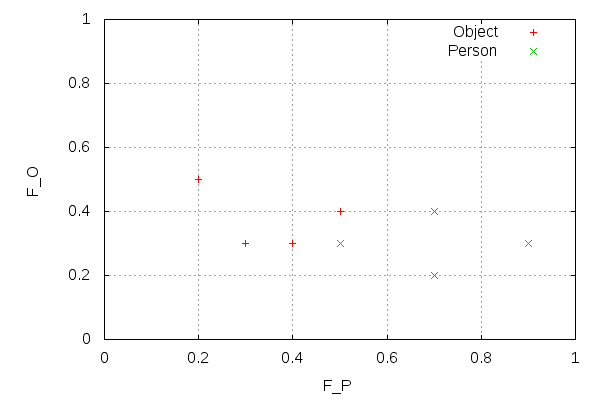
\includegraphics[scale=0.5]{pics/svm_training}
	\end{tabular}
	\caption{Mögliche Visualisierung der SVM nach dem Trainingsschritt ohne Hyperebene}
	\label{tab:svm_training}
\end{table}\\
Nachdem sich die Eigenschaften von Personen und Objekten hoffentlich etwas unterscheiden und die verschiedenen Typen im Diagramm getrennt erscheinen, muss man nun noch eine Hyperebene mit möglichst großem Abstand zum Rand zwischen den aufgetrennten Typen einfügen. Dafür wurde im Paper über ``A 2-Poisson Model for Probabilistic Coreference of Named Entities for Improved Text Retrieval'' \cite{paper:Na} eine Radial Basis Function herangezogen. 




\newpage
%%%%%%%%%%%%%%%%%%%%%%%%%%%%% <Feedback-Based Identification> %%%%%%%%%%%%%%%%%%%%%
\subsection{Automatische Erkennung von Koreferenzen}
Da die Menge an Koreferenzen 
\[A_O=\left\{\text{'it', 'its'}\right\}\]
für Objekte nicht ausreichend ist, haben die Autoren des Papers \NaNg\cite{paper:Na} ein Verfahren entwickelt, um die Menge $A_O$ zu erweitern. Sie nennen ihren Algorithmus ``Feedback-Based Identification of Anaphoric Expressions''.



%%%%%%%%%%%%%%%%%%%%%%%%%%%%% <Retrieval Method> %%%%%%%%%%%%%%%%%%%%%%%%%%%%%%%%%%
\subsection{Retrieval Method}


\section{Evaluation}
Im Paper \NaNg\cite{paper:Na} wurden noch verschiedene Performancetests durchgeführt. Dafür wurde die TREC Blog Sammlung verwendet. Die meisten Suchanfragen darin sind Eigennamen. Davon sind 33 Personenentitäten und 108 Objekte. Die restlichen 9 Suchanfragen sind allgemeiner Natur. Von den 150 Queries wurden 50 Suchanfragen als Trainingsmenge zum Parametertuning verwendet und die restlichen 100 Queries zum Testen.\\
Die Support Vector Machine Klassifikatoren wurden ebenfalls mit 50 Queries eingestellt. Damit konnten von den verbleibenden 100 Suchanfragen 93 richtig einem Objekt oder einer Person zugeordnet werden. Von den 7 falsch klassifizierten Suchanfragen wurden 4 Objekte als Personen erkannt und 3 Personen als Objekte.\\
Zuletzt wurden verschiedene Testläufe mit verschiedenen Modellen gestartet:
\begin{itemize}
	\item \textbf{REF}: Hierfür wurde die raw entity frequency im vorgestellten Retrieval Modell verwendet.
	\item \textbf{CEEF-Thr}: Das Ranking wurde mit dem Coreferntial Enhanced Entity Frequency Modell nach dem threshold Ansatz durchgeführt.
	\item \textbf{CEEF-2Poisson}: Ranking mit CEEF-Modell. Die möglichen Koreferenzen beschränkten sich dabei auf die Mengen\\
$A_P=\left\{ \text{'he', 'she', 'his', 'her', 'himself', 'herself'} \right\}$ und
$A_0=\left\{ \text{'it', 'its'} \right\}$.
	\item \textbf{CEEF-FB-2Poisson}: Die möglichen Koreferenzen wurden mit dem unter ``Automatische Erkennung von Koreferenzen'' vorgestellten Verfahren von Seung-Hoon Na und Hwee Tou Ng ermittelt. Mit den so erhaltenen Mengen an Koreferenzen wurde das CEEF-Modell angewandt.
	\item \textbf{CEEF-FB-2Poisson*}: Hier wurde das CEEF-Model mit der ``Feedbackbased Identification'' verwendet. Allerdings wurden die Entitäten nicht mit dem Support Vector Machine Klassifikator Personen oder Objekten zugeordnet, sondern per Hand.
\end{itemize}
\begin{table}[h]
	\centering
	\begin{tabular}{lS[tabnumalign=centre,tabformat=1.4,decimalsymbol=comma]S[tabnumalign=centre,tabformat=1.4,decimalsymbol=comma]S[tabnumalign=centre,tabformat=1.4,decimalsymbol=comma]}
		\toprule
		Methods & {MAP} & {Pr@5} & {Pr@10}\\
		\midrule
		REF & 0.3929 & 0.6707 & 0.6616\\
		CEEF-Thr & 0.3968 & 0.6788 & 0.6778\\
		CEEF-2Poisson & 0.4139 & 0.7060 & 0.6940\\
		CEEF-FB-2Poisson & 0.4165 & 0.7320 & 0.7200\\
		CEEF-FB-2Poisson* & 0.4177 & 0.7420 & 0.7270\\
		\bottomrule
	\end{tabular}
	\caption{Comparison of MAP, Pr@5, Pr@10}
	\cite{paper:Na}
\end{table}
In der ersten Tabelle sieht man die einzelnen Methoden im direkten Vergleich. Als Testmaß verwendete man MAP, die Mean Average Precision, Pr@5, die Präzision für die besten 5 Dokumente und Pr@10, die Präzision für die besten 10 Dokumente. In MAP sind alle CEEF-Modelle signifikant besser als REF.\\
Bei Pr@5 und Pr@10 sind nur noch die CEEF-Poisson-Methoden signifikant besser als REF. Diese Tatsache ist in dem Orginalpaper \NaNg\cite{paper:Na} schön dargestellt.\\
\begin{table}[h]
	\centering
	\begin{tabular}{lS[tabnumalign=centre,tabformat=1.4,decimalsymbol=comma]S[tabnumalign=centre,tabformat=1.4,decimalsymbol=comma]}
		\toprule
		Methods & {LM} & {LMFB} \\
		\midrule
		B (Baseline Run) & 0.4043 & 0.4254 \\
		B+REF & 0.4665 & 0.4868 \\
		B+CEEF-Thr & 0.4831 & 0.4942 \\
		B+CEEF-2Poisson & 0.4874 & 0.5000 \\
		B+CEEF-FB-2Poisson & 0.5074 & 0.5090 \\
		B+CEEF-FB-2Poisson* & 0.5087 & 0.5106 \\
		\bottomrule
	\end{tabular}
	\caption{Comparison of MAP of REF and CEEF methods combining with Language Models \cite{paper:Zhai1}\cite{paper:Zhai2}}
	\cite{paper:Na}
\end{table}\\
\\
In der 2. Tabelle wird die Kombination der vorgestellten Methoden mit Language Modelling-Methoden \cite{paper:Zhai1}\cite{paper:Zhai2} getestet. Dabei ist zu sehen, dass die Mean Average Precision gewaltig gesteigert werden kann im Vergleich zu den unkombinierten Methoden.
%Paper einfügen, wie wann und warum man das macht
\begin{table}[h]
	\centering
		\begin{tabular}{lS[tabnumalign=centre,tabformat=1.4,decimalsymbol=comma]S[tabnumalign=centre,tabformat=1.4,decimalsymbol=comma]S[tabnumalign=centre,tabformat=1.4,decimalsymbol=comma]S[tabnumalign=centre,tabformat=1.4,decimalsymbol=comma]}
			\toprule
			Query Type & {REF} & {CEEF} & {CEEF-FB} & {CEEF-FB*}\\
			\midrule
			Person & 0.5640 & 0.5793 & 0.5761 & 0.5781\\
			Company, etc. & 0.5061 & 0.5170 & 0.5305 & 0.5305\\
			Product & 0.5245 & 0.5401 & 0.5680 & 0.5680\\
			TV program, etc & 0.3664 & 0.3754 & 0.3793 & 0.3994\\
			Organization & 0.4468 & 0.4682 & 0.4701 & 0.4701\\
			Event, etc. & 0.5039 & 0.4987 & 0.5012 & 0.5021\\
			Other Types & 0.4785 & 0.4889 & 0.5040 & 0.5040\\
			Topic & 0.2754 & 0.3078 & 0.3094 & 0.3123\\
			All & 0.4868 & 0.5000 & 0.5090 & 0.5106\\
			\bottomrule
		\end{tabular}
		\caption{Comparison of MAP of REF and CEEF methods, combining with LMFB each query type.\cite{paper:Na}}
\end{table}\\
In Tabelle 3 kann man sehr schön sehen, dass das angewendete Verfahren für Personen-Queries immernoch am besten funktioniert.

\begin{table}[h]
	\centering
	\begin{tabular}{lS[tabnumalign=centre,tabformat=1.4,decimalsymbol=comma]S[tabnumalign=centre,tabformat=1.4,decimalsymbol=comma]S[tabnumalign=centre,tabformat=1.4,decimalsymbol=comma]S[tabnumalign=centre,tabformat=1.4,decimalsymbol=comma]}
		\toprule
		Query Type & {NONE} & {REF} & {CEEF} & {CEEF-FB}\\
		\midrule
		TREC '07 & 0.5406 & 0.5569 & 0.5646 & 0.5733\\
		TREC '08 & 0.5032 & 0.5216 & 0.5248 & 0.5330\\
		\bottomrule
	\end{tabular}
	\caption{Comparison of MAP of TREC08BEST and others. NONE means non-combined baseline run.}
	\cite{paper:Na}
\end{table}



% References (Literaturverzeichnis):
% a) Style (with abbreviations: use alpha):
\bibliographystyle{plainnat-d}
% b) The File:
\newpage
\bibliography{seminararbeit}

\end{document}
\end{document}
\end{document}
\end{document}
